\section{CLogger Class Reference}
\label{classCLogger}\index{CLogger@{CLogger}}
{\tt \#include $<$CLogger.hpp$>$}

Inheritance diagram for CLogger::\begin{figure}[H]
\begin{center}
\leavevmode
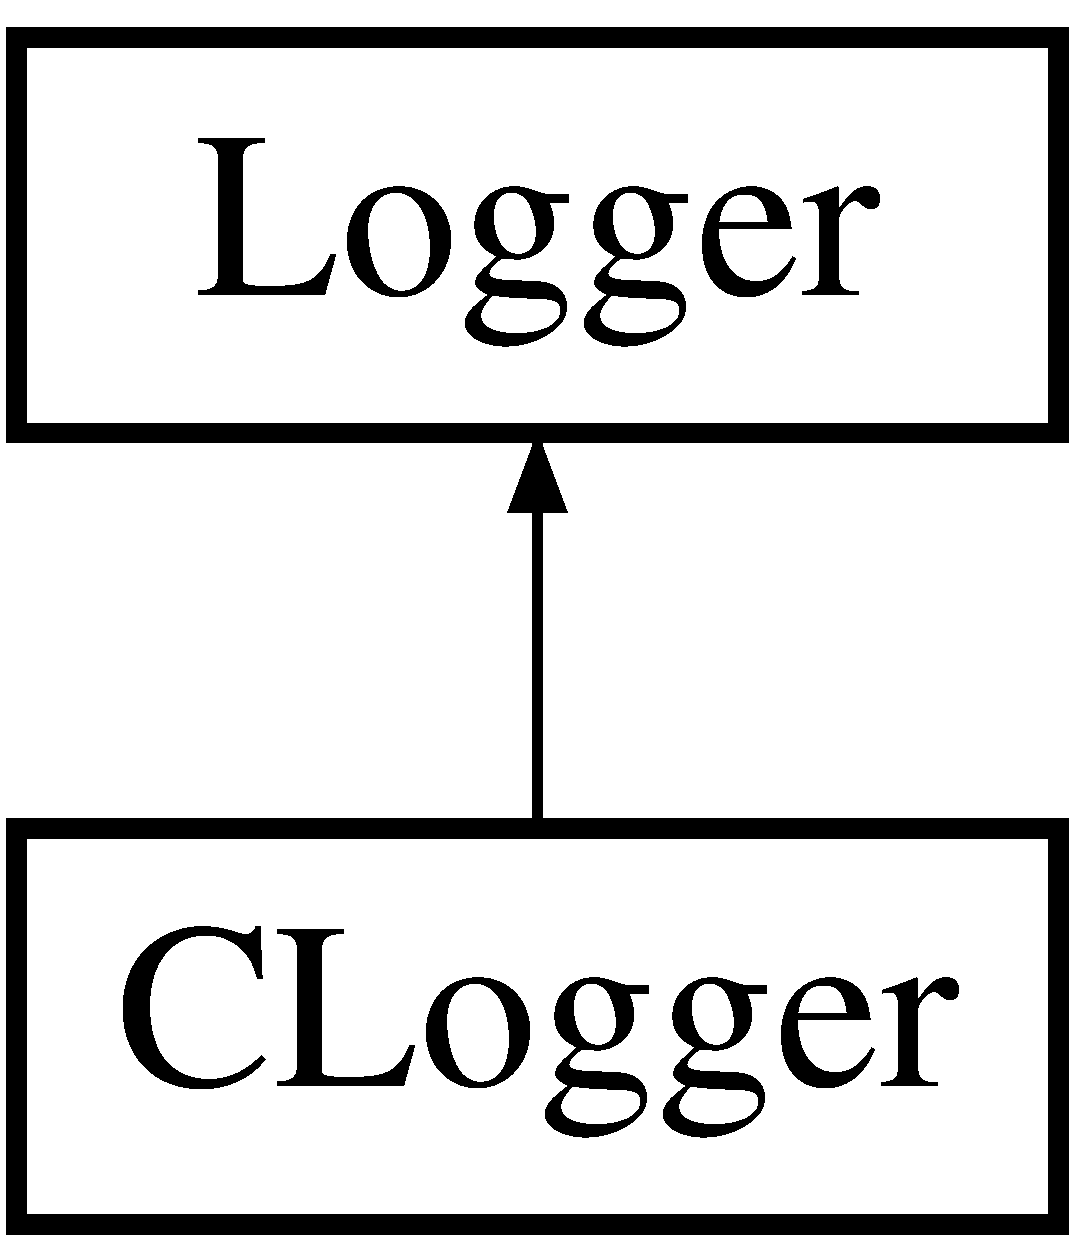
\includegraphics[height=2cm]{classCLogger}
\end{center}
\end{figure}
\subsection*{Public Member Functions}
\begin{CompactItemize}
\item 
{\bf CLogger} (FILE $\ast$\&log, int n\-Log\-Level=ERROR\_\-MESSAGES\_\-LR, bool close\-On\-Exit=false)\label{classCLogger_a0}

\item 
virtual void {\bf log} (int level=ERROR\_\-MESSAGES\_\-LR, const string \&message=\char`\"{}\char`\"{}) const 
\end{CompactItemize}


\subsection{Detailed Description}
Provides an interface to log to a FILE$\ast$.



\subsection{Member Function Documentation}
\index{CLogger@{CLogger}!log@{log}}
\index{log@{log}!CLogger@{CLogger}}
\subsubsection{\setlength{\rightskip}{0pt plus 5cm}void CLogger::log (int {\em level} = {\tt ERROR\_\-MESSAGES\_\-LR}, const string \& {\em message} = {\tt \char`\"{}\char`\"{}}) const\hspace{0.3cm}{\tt  [virtual]}}\label{classCLogger_a2}


Description: Tests the log level of the message and reports the message if it has a high enough priority otherwise the message is suppressed.

Implements {\bf Logger} {\rm (p.\,\pageref{classLogger_a2})}.

The documentation for this class was generated from the following files:\begin{CompactItemize}
\item 
CLogger.hpp\item 
CLogger.cpp\end{CompactItemize}
